\documentclass[a4paper,12pt]{report}
\def\magyarOptions{defaults=hu-min}

\usepackage[magyar]{babel}
\usepackage{t1enc}
\usepackage{indentfirst}
\usepackage[utf8]{inputenc}
\usepackage{url}
\usepackage{times}
\usepackage{subfigure}
\usepackage{amsmath}
\usepackage{amssymb}
\usepackage{amsthm}
\usepackage{verbatim}
\usepackage{fancyhdr}
\usepackage{graphicx}
\usepackage{psfrag}
\usepackage{setspace}
\usepackage[numbers]{natbib}
\usepackage{color}
\usepackage{xcolor}
\usepackage{listings}
\usepackage{todonotes}
\usepackage{rotating}
\usepackage{siunitx}

\bibliographystyle{abbrvnat}

\hoffset -0.85in
\voffset -1.5in
\oddsidemargin 30mm
\evensidemargin 20mm
\textwidth 150mm
\topmargin 30mm
\textheight 237mm
\onehalfspacing

\definecolor{codegreen}{rgb}{0,0.6,0}
\definecolor{codegray}{rgb}{0.5,0.5,0.5}
\definecolor{codepurple}{rgb}{0.58,0,0.82}
\definecolor{backcolour}{rgb}{0.95,0.95,0.92}
 
\lstdefinestyle{mystyle}{
    backgroundcolor=\color{backcolour},   
    commentstyle=\color{codegreen},
    keywordstyle=\color{magenta},
    numberstyle=\tiny\color{codegray},
    stringstyle=\color{codepurple},
    basicstyle=\footnotesize,
    breakatwhitespace=false,         
    breaklines=true,                 
    captionpos=b,                    
    keepspaces=true,                 
    numbers=left,                    
    numbersep=5pt,                  
    showspaces=false,                
    showstringspaces=false,
    showtabs=false,                  
    tabsize=2
}
\renewcommand{\lstlistingname}{Forráskód}
\lstset{style=mystyle}

%%%%%%%%%%%%%%%%%%%%%%%%%%%%%%%%%%%%%%%%%%%%%%%%%%%%%%

\begin{document}

\begin{singlespace}

\fancypagestyle{plain}{
\fancyhf{}
\fancyfoot[R]{\thepage}
\renewcommand{\headrulewidth}{0pt}
}

\pagestyle{fancy}
\fancyhf{}
\fancyhead[R]{Valós idejű rendőr-ágens irányító a Robocar World Championshiphez}
\fancyfoot[R]{\thepage}

\thispagestyle{empty}

\begin{center}
\vspace*{1cm}
{\Large\bf Debreceni Egyetem}
\vspace{0.2cm}

{\Large\bf Informatikai Kar}
\vspace{0.2cm}

{Információ Technológia Tanszék}
\vspace*{2.8cm}

{\LARGE\bf Valós idejű rendőr-ágens irányító a Robocar World Championshiphez}
\vspace*{6cm}


{\large
\begin{tabular}{c@{\hspace{3cm}}c}
\emph{Témavezető:}      &       \emph{Készítette:}\\
\bf{dr. Bátfai Norbert} &       \bf{Balkus Gergő Máté}\\
egyetemi adjunktus      &        programtervező informatikus hallgató\\
\end{tabular}
}

\vspace*{1cm}

\begin{center}
{\large
\begin{tabular}{c}
\vspace{5mm}
{A dolgozat benyújtásához hozzájárulok.}\\

\makebox[3in]{\hrulefill}  \\
dr. Bátfai Norbert\\
\end{tabular}
}
\end{center}

\end{center}

\vspace{25mm}
\begin{center}
{\Large
Debrecen
\\
\vspace{2mm}
2016
}
\end{center}

\tableofcontents

\end{singlespace}
%%%%%%%%%%%%%%%%%%%%%%%%%%%%%%%%%%%%%%%%%%%%%%%%%%%%%%%%%%%%%%%%%%%%%%%%%%%%%%%%%%%%%%%%%%%%%%%%%%%%%%%%%%%%%%%%%%%%%%%%%%%

\chapter{Bevezetés}

\section{Robotautók}
\label{robocars}

\begin{figure}[h]
\centerline{
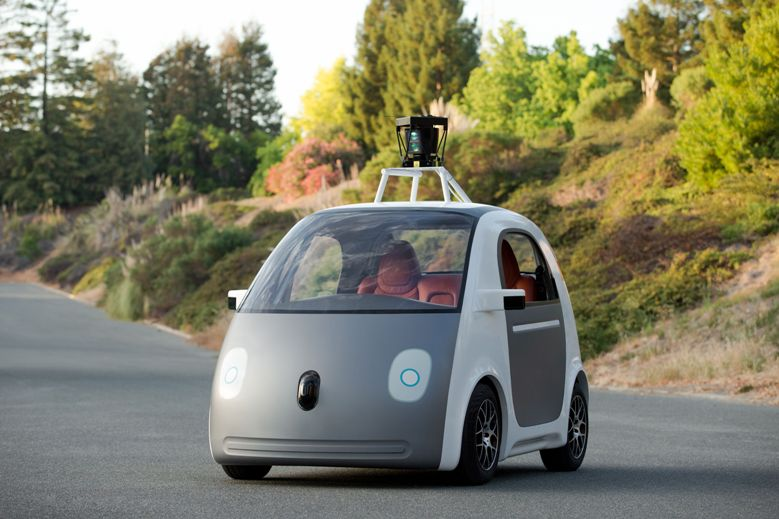
\includegraphics[width=6in]{img/googleauto}}
\caption{A Google által fejlesztett robotautó. Forrás: \cite{googlecarimage}.}
\label{googleauto}
\end{figure}

TODO

\section{Okos városok}
\label{smartcities}

TODO


\chapter{A Robocar World Championship (OOCWC)}
\label{oocwc}

\section{Ismerkedés az OOCWC rendszerrel}

Az OOCWC rendszer célja, hogy az autonóm autók és az okos városok közötti összefüggéseket vizsgálja, kutatási valamint oktatási célokat is szolgál. A rendszer felépítését a 2.1. ábra szemlélteti.

\begin{figure}[h]
\centerline{
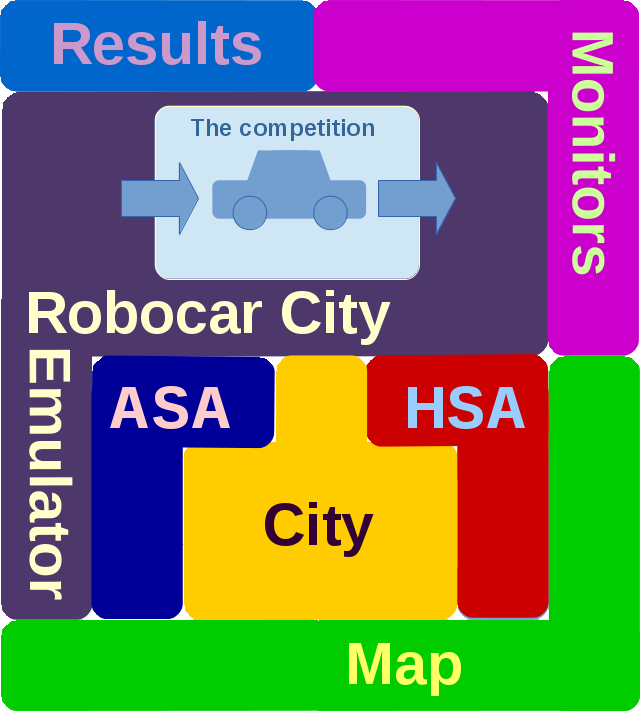
\includegraphics[width=3.5in]{img/tetris_plan}}
\caption{Az OOCWC rendszer tetris terve. Forrás: \cite{oocwcrepo}.}
\label{basedesign}
\end{figure}

Ez alapján a rendszer egyes elemei:

\begin{itemize}
\item Map -- a szimuláció egy adott térképen értelmezett,
\item City -- a szimuláció működési egysége,
\item The competition -- a verseny célja / maga a verseny,
\item ASA -- automatikus adatgyűjtő rendszer,
\item HSA -- kézi adatgyűjtő rendszer,
\item Robocar City Emulator -- forgalom emuláció,
\item Results -- a verseny eredményei, illetve kísérletek eredményei,
\item Monitors -- megjelenítők, vizualizáció.
\end{itemize}

A rendszer többcélú. Egyrészt egy kutatási platformot kínál forgalomelemzésre, szimulációkra. A szimuláció az OpenStreetMap \cite{osm} térképein fut. 

\vspace{2mm}
A rendszer másik célja, hogy egy verseny segítségével találjuk meg a lehető legjobb forgalomirányító algoritmust. Az OOCWC már több sikeres versenyen is túl van a Debreceni Egyetem Informatikai Karán \cite{competitions}. Gyakori, hogy egy kutatás által létrejött rendszerre versenyt szerveznek a felhasználók körében. Erre egy jó példa az mesterséges intelligencia (AI - Artificial Intelligence) területén a RoboCup \cite{robocup}.

\vspace{2mm}
Fontos megemlíteni, hogy a Robocar World Cup kiválóan alkalmazkodik a különböző esetekre. Az oktatás és kutatások támogatására került kifejlesztésre a ``Police Edition'' (egy pillanatkép ebből a változatból a \ref{police}. ábrán látható). A cél, hogy rendőr-ágensekkel, melyeket a felhasználó által megírt irányító algoritmus vezérel, minél több gengszter-ágenst kapjunk el.

\vspace{2mm}
A rendszer jelenleg háromféle forgalmi egységet különböztet meg, routine cars, smart cars és guided cars. A szimuláció kezdőállapota a routine cars és smart cars elhelyezése a térképen a gyűjtött adatok alapján.

\begin{figure}[h]
\centerline{
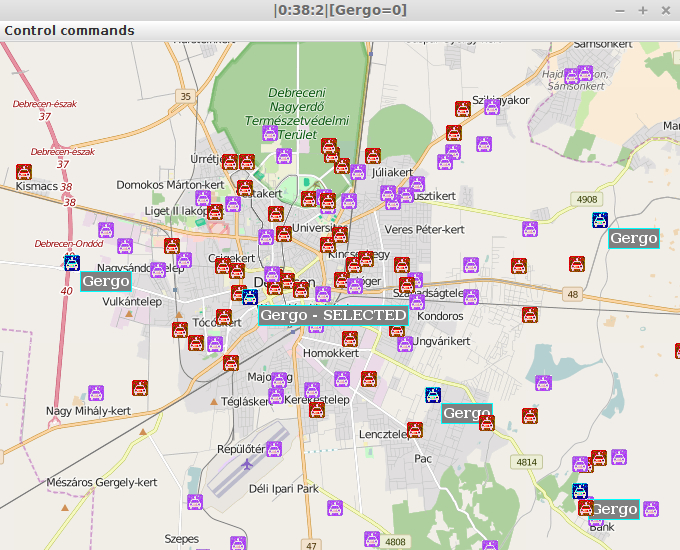
\includegraphics[width=6in]{img/copselected}}
\caption{Pillanatkép a rendszer ``Police Edition'' változatának a projekt szerinti módosításával (lásd: \ref{theapp}. fejezet). A térkép az OSM egy részlete, Debrecen, Hajdú-Bihar Megye, Magyarország. A megjelenítést a JXMapViewer2 \cite{jxmapv} biztosítja. A térképen a routine car rózsaszínnel, a gengszter ágensek pirossal (smart car), a rendőrágensek (guided car) kékkel jelölve. Az éppen kiválasztott rendőr-ágens melyet éppen irányítunk pedig el van látva a ``SELECTED'' felirattal. Forrás: \cite{infocomjournal} 
\label{police}}
\end{figure}

\vspace{2mm}
A rendszer ``Police Edition'' változatából készíthetnek egy saját fork-ot a hallgatók és az érdeklődő kutatók. A játék célja, hogy a rendőr ágensekkel minél több gengszter ágenst kapjunk el. A bemutatott projekt (\ref{theapp}. fejezet) is egy ilyen forknak tekinthető.

\section{A rendszer elindítása}
\label{howtostart}

TODO parancsok berakása és megmagyarázása

\section{Szükséges módosítások a projekt számára}
\label{changes}

\subsection{Az eredeti irányítás}
\label{originalrouting}
Eredetileg a rendőr-ágensek is C++ nyelven (\ref{cplusplus}. fejezet) lettek megvalósítva, ezáltal hozzáférnek az OOCWC osztott memóriájához (shared memory), amiben több adat közt megtalálható az OSM \citep{osm} (\ref{osm}. fejezet) térképből felépített irányított gráf BGL (Boost Graph Library) (\ref{boost}. fejezet). Ezt a gráfot és a Boost, gráfokra implementált, kereső algoritmusait felhasználva a rendőr-ágens képes létrehozni a szimulációs szerver által értelmezhető útkereső (routing) parancsot, mellyel a szerver a kapott parancs alapján mozgatja a megfelelő rendőr-ágenst. 

\vspace{2mm}
TODO a parancs szintaxisának bemutatása

TODO forráskód a routingról

\subsection{Az új irányítás}
\label{newrouting}

Ahhoz hogy az eredeti irányításhoz hasonló mozgatást érjünk el a kívánt rendőr-ágensen, egy olyan programozási nyelvvel amelynek nincs hozzáférése az OOCWC által felépített osztott memóriához, egy új parancs bevezetésére volt szükség, amely helyettesíti az eredeti útkereső parancsot, a valódi routingot (az út megtalálását kettő csomópont között) pedig a szerverre kellett bízni.

\vspace{2mm}
TODO az új parancs szintaxisának bemutatása

TODO forráskód az új routingról

\section{Az adat áramlása}
\label{dataflow}

\begin{figure}[h]
\centerline{
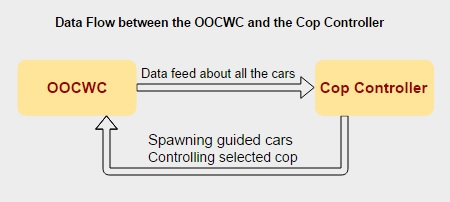
\includegraphics[width=4.5in]{img/dataflow}}
\caption{Az adat áramlása az OOCWC rendszer (\ref{oocwc}. fejezet) és az alkalmazás (\ref{theapp}. fejezet) között.} 
\label{dataflowpicture}}
\end{figure}

\newpage
\chapter{Felhasznált technológiák}
\label{technologies}

\section{Java}
\label{java}

A Java egy általános célú, objektumorientált programozási nyelv, amelyet a Sun Microsystems fejlesztett az 1990-es évek elejétől kezdve egészen 2009-ig, amikor a céget felvásárolta az Oracle. 2011-ben a Java 1.7-es verzióját, 2014-ben pedig az 1.8-as verzióját már az új tulajdonos gondozásában adták ki.

\lstinputlisting[language=Java, caption=A klaszzikus ``Hello World!'' Javában, label=helloworldjava]{src/helloworld.java}

\vspace{2mm}
A nyelv 2016-ban is sikeres a szerver oldalon a servlet, a JSP és Enterprise JavaBeans, JDBC technológiákkal, integrációs lehetőségeivel, nyelvi eszközeivel, jvm nyelveivel és a nyílt forráskódú közösség tudására is építve.

\vspace{2mm}
A Java alkalmazásokat jellemzően bájtkód formátumra alakítják, de közvetlenül natív (gépi) kód is készíthető Java forráskódból. A bájtkód futtatása a Java virtuális géppel történik, ami vagy interpretálja a bájtkódot, vagy natív gépi kódot készít belőle, és azt futtatja az adott operációs rendszeren. Létezik közvetlenül Java bájtkódot futtató hardver is, az úgynevezett Java processzor.

\vspace{2mm}
A Java nyelv a szintaxisát főleg a C és a C++ (\ref{cplusplus}. fejezet) nyelvektől örökölte, viszont sokkal egyszerűbb objektummodellel rendelkezik, mint a C++. Példaként szolgál az egyik fő különbsége a C++ nyelvtől: nincs az osztályok között többszörös öröklődés (ezt a célt az interfészek valósítják meg). 

\vspace{2mm}
A JavaScript szintaxisa és neve hasonló ugyan a Java-éhoz, de a két nyelv nem áll olyan szoros rokonságban, mint azt ezekből a hasonlóságokból gondolhatnánk.

\vspace{2mm}
Négy fontos szempontot tartottak szem előtt, amikor a Javát kifejlesztették:
\begin{itemize}
\item objektumorientáltság;
\item függetlenség az operációs rendszertől amelyen fut (platformfüggetlenség);
\item olyan kódokat és könyvtárakat tartalmazzon, amelyek elősegítik a hálózati programozást;
\item távoli gépeken is képes legyen biztonságosan futni.
\end{itemize}

\subsection{Története}
\label{javahistory}
\vspace{2mm}
Bár a nyelv neve kezdetben Oak (tölgyfa) volt, (James Gosling, a nyelv atyja nevezte így az irodája előtt növő tölgyfáról), később kiderült, hogy ilyen elnevezésű nyelv már létezik, ezért végül Java néven vált ismertté. A Java nyelvet kávézás közben találták ki, innen ered a kávéscsésze ikon \cite{javaname}.

\subsection{Objektumorientáltság}
\label{oo}

A nyelv első tulajdonsága, az objektumorientáltság (``OO''), a programozási stílusra és a nyelv struktúrájára utal. Az OO fontos szempontja, hogy a szoftvert ``dolgok'' (objektumok) alapján csoportosítja, nem az elvégzett feladatok a fő szempont. Ennek alapja, hogy az előbbi sokkal kevesebbet változik, mint az utóbbi, így az objektumok (az adatokat tartalmazó entitások) jobb alapot biztosítanak egy szoftverrendszer megtervezéséhez. A cél az volt, hogy nagy fejlesztési projekteket könnyebben lehessen kezelni, így csökken az elhibázott projektek száma.

\subsection{Platformfüggetlenség}
\label{platformfugg}

Ez a tulajdonság azt jelenti, hogy a Java-ban írt programok a legtöbb hardveren ugyanúgy futnak. Ezt úgy érik el, hogy a Java fordítóprogram a forráskódot csak egy úgynevezett Java bájtkódra fordítja le. Léteznek továbbá szabványos könyvtárcsomagok, amelyek, - közvetítve a kód és a gép között, - egységes funkcionalitásként teszik elérhetővé az illető hardver sajátságosságait (grafika, szálak és hálózat).

\vspace{2mm}
Vannak olyan Java fordítóprogramok, amelyek a forráskódot natív gépi kódra fordítják le, - ilyen például a GCJ, - ezzel valamelyest felgyorsítva annak futtatását. Cserébe a lefordított program elveszíti hordozhatóságát.

\vspace{2mm}
Egyes cégek, mint például a Microsoft, mégis platformfüggő sajátságokat adtak a nyelvhez, amire a Sun keményen reagált: beperelte a Microsoftot (az amerikai bíróság 20 millió dollár kártérítésre és a sajátos tulajdonságok visszavonására kötelezte a céget). Válaszként a Microsoft kihagyta a Java rendszert a jövőbeli termékekből és Windows-változatokból. Ez azt jelenti, hogy az Internet Explorer webböngésző alapváltozataiból hiányzik a Java. Így abban az olyan weboldalak, amelyek Java-t használnak, nem fognak helyesen megjelenni. A Windows-felhasználók e problémáját megoldva a Sun és más cégek ingyenesen letölthetővé tették a JVM rendszert azon Windows-változatok számára, amelyekből a virtuális gép hiányzik.

\vspace{2mm}
A hordozhatóság megvalósítása technikailag nagyon bonyolult. E közben a Java esetében is sok vita volt. Az „írd meg egyszer, futtasd bárhol” szlogenből „írd meg egyszer, keress hibát mindenhol” lett. 2016-ra a hordozhatóság nem okoz tovább problémát, mivel maga a Java is nyílt szabványokra épül, például: openGL, vagy Open POSIX.

\vspace{2mm}
A Java minden jelentősebb platformon elérhető (Linux, Unix, Windows, iOS).

\subsection{Swing}
\label{swing}

A Swing egy eszközkészlet a grafikus felhasználói felületek létrehozására.

\vspace{2mm}
A Swinget azzal a céllal fejlesztették, hogy egy szofisztikáltabb GUI komponenshalmazt szolgáltasson mint a korábbi Abstract Window Toolkit (AWT) \cite{awt}. A Swingnek a komponensei erőteljesebb és flexibilisebb az AWT-hez hasonlítva. A már ismert komponensekhez, mint például a Button-ök, check boxok és labelek, a Swing olyan további fejlett eszközökkel szolgál, mint a tabbed panel, scroll pane, fák, táblázatok és listák.

\vspace{2mm}
Ellentétben az Abstract Window Toolkit komponenseivel, a Swing komponensei nem platform-specifikus kódként lettek implementálva. Helyette teljesen Java nyelven írták meg, ezáltal a komponensek platform-függetlenek lettek. A ``lightweight'' kifejezéssel írjuk le az ilyen elemeket \cite{swingarticle}.

\vspace{2mm}
A Swinget a közeljövőben a JavaFX \cite{javafx} fogja felváltani.

\subsection{JXMapViewer}
\label{jxmapviewer}

A JXMapViewer \cite{jxmapv} egy nyílt forráskódú Java könyvtár, ami egy Swing (\ref{swing}. fejezet) JPanelt \cite{jpanel} szolgáltat, melynek feladata a térkép betöltése, és mutatása.

\vspace{2mm}
TODO

\newpage
\section{C++}
\label{cplusplus}

A C++ egy általános célú, magas szintű programozási nyelv. Támogatja a procedurális, az objektumorientált és a generikus programozást is. Napjainkban szinte minden operációs rendszer alá létezik C++ fordító. A nyelv a C hatékonyságának megőrzése mellett törekszik a könnyebben megírható, karbantartható és újrahasznosítható kód írására, ez azonban sok kompromisszummal jár. Erre utal, hogy általánosan elterjedt a mid-level minősítése is, bár szigorú értelemben véve egyértelműen magas szintű.

\vspace{2mm}
A nyelv tervezésénél fontos szempont volt a C-vel való kompatibilitás, ezt oly mértékben sikerült megvalósítani, hogy minden szintaktikailag helyes C program egyben egy szintaktikailag helyes C++ program is. 

\lstinputlisting[language=C++, caption=A klaszzikus ``Hello World!'' C++-ban, label=helloworldcpp]{src/helloworld.cpp}

\subsection{Története}
\label{cpphistory}

Bjarne Stroustrup kezdte el a C++ programozási nyelv fejlesztését a C programozási nyelv kiterjesztéseként, más nyelvekből véve át megoldásokat, ötleteket. A nyelv első, nem kísérleti körülmények közt való használatára 1983-ban került sor, 1987-ben pedig nyilvánvalóvá vált, hogy a C++ szabványosítása elkerülhetetlen. Ez a folyamat 1991 júniusában kezdődött el, amikor az ISO szabványosítási kezdeményezés részévé vált. A C++ programozási nyelv szabványát 1998-ban hagyták jóvá ISO/IEC 14882:1998 \cite{c++98} (C++98) néven, a 2003-as változat kódjelzése pedig a ISO/IEC 14882:2003 \cite{c++03} (C++03) lett. Az ezt követő 2011-es változatot ISO/IEC 14882:2011 \cite{c++11} (C++11) kódjelzéssel hagyták jóvá. A jelenlegi legfrissebb változata a 2014-es ISO/IEC 14882:2014 \cite{c++14} (C++14) kódjelzésű verzió. 

\subsection{Boost library}
\label{boost}

\begin{figure}[h]
\centerline{

\includegraphics[width=3.6in]{img/boost}}
\caption{A Boost logója. Forrás: \cite{boostlogo}.}
\label{basedesign}
\end{figure}

\vspace{2mm}
A Boost a C++ programozási nyelvhez ad támogatást olyan könyvtárakkal, melyek különböző területek különböző problémáit segítenek megoldani. Többek között ilyen területek a lineáris algebra, a pseudorandom számok generálása, a többszálasítás, a képfeldolgozás, a reguláris kiejezések, illetve a unittesztelés. 

\vspace{2mm}
Az OOCWC (\ref{oocwc}. fejezet) számára az egyik legfontosabb ilyen könyvtár a BGL (Boost Graph Library) \cite{bgl}, melynek segítségével épül fel az OpenStreetMap \cite{osm} (\ref{osm}. fejezet) térkép alapján az OOCWC irányított gráfja.

\newpage
\section{Maven}
\label{maven}

Az Apache Maven (röviden Maven) egy szoftver, amelyet szoftverprojektek menedzselésére és a build folyamat automatizálására lehet használni. Jason van Zyl készítette 2002-ben. Funkcionalitásában hasonlít az Apache Ant eszközhöz. A projektet az Apache Software Foundation hosztolja, ahol korábban a Jakarta Projekt részeként működött.

\vspace{2mm}
A Maven bevezeti a POM, azaz a Projekt Objektummodell (angolul: Project Object Model) fogalmát. Egy POM egy buildelendő projektet ír le és annak függőségeit. Az egyes lépéseket céloknak, angolul goal-oknak nevezik. Vannak előre definiált célok a tipikus feladatokra, mint például a kód fordítása és csomagolása, de a felhasználónak lehetősége van saját célokat is definiálni a projektspecifikus lépések végrehajtására.

\vspace{2mm}
A Maven hálózatképes, tehát szükség esetén dinamikusan is le tud tölteni komponenseket. Repository névvel illetik a különböző hosztok fájlrendszereinek azon mappáit, ahol a letölthető komponensek találhatók. A Maven nem csak a repository-kból való letöltést támogatja, hanem a készült szoftvercsomag feltöltését is. Ezzel az automatizálható le- és feltöltési mechanizmussal a Maven de facto szabványt próbál teremteni, de elég lassan fogadja el a Java közösség.

\vspace{2mm}
A Maven-nek léteznek beépülő moduljai számos népszerű IDE-höz, melyek integrációt nyújtanak a Mavennal való az IDE build mechanizmusához, kódszerkesztő eszközeihez. Ezekkel lehetőség van az IDE-ből lefordítani a projekteket, és beállítani a classpath-t a kód kiegészítéshez ill. fordító hibák színezéséhez stb. Ilyen IDE például az Eclipse, illetve a NetBeans is.

\newpage
\section{Git}
\label{git}

A Git egy nyílt forráskódú, elosztott verziókezelő szoftver, vagy másképpen egy szoftverforráskód-kezelő rendszer, amely a sebességre helyezi a hangsúlyt. A Gitet eredetileg Linus Torvalds fejlesztette ki a Linux kernel fejlesztéséhez. Minden Git munkamásolat egy teljes értékű repository teljes verziótörténettel és teljes revíziókövetési lehetőséggel, amely nem függ a hálózat elérésétől vagy központi szervertől.

\vspace{2mm}
Számos nagy volumenű projekt használja jelenleg a Gitet verziókezelő rendszerként; a legfontosabbak ezek közül: Linux-rendszermag, GNOME, Samba, X.org, Qt. A Git karbantartásának felügyeletét jelenleg Junio Hamano látja el.

\vspace{2mm}
A Git rendszerét a BitKeeper és a Monotone ihlette. Eredetileg alacsony szintű verziókövető rendszernek tervezték, azonban teljes értékű revíziókövető rendszerré szélesedett, amelyet már közvetlenül is lehet használni. Torvalds, aki jártas a nagy, szétosztott fejlesztési projektekben és a fájlrendszerekben, és gyorsan akart működő rendszert fejleszteni, ezekre az elvekre alapozta a Gitet:

\begin{itemize}
\item A nemlineáris fejlesztés erős támogatása. A Git támogatja az ágak (branchek) készítését, összefésülésüket, és tartalmaz eszközöket a nem-lineáris fejlesztési történet ábrázolására.
\item Elosztott fejlesztés. A Git minden fejlesztő helyi munkaváltozatában rendelkezésre bocsátja a teljes addigi fejlesztési történetet, és a változtatások másolása mindig két repository között történik. Ezeket a változtatásokat, mint külön ágakat importálják és összefésülhetőek, hasonlóan a helyben létrehozott fejlesztési branchokhoz.
\item Nagy objektumok hatékony használata.
\item Kriptográfiailag hitelesített történet. A Git-történet olyan módon tárolódik, hogy a szóban forgó revízió neve függ a hozzá vezető fejlesztési történettől. Ha egyszer publikálták, akkor már nem lehetséges észrevétlenül megváltoztatni egy régi revíziót. A struktúra hasonlatos a hash-fához, de hozzáadott adatokkal az egyes csomópontokon és leveleken.
\item Eszközkészlet-szerű megoldás. A Git maga C-ben írt programok halmaza, számos shell-szkripttel megtűzdelve, amelyek összefűzik ezeket a C-ben írt programokat. Annak ellenére, hogy a szkriptek többségét újraírták C-ben a Microsoft Windowsra való portolás eredményeként, a struktúra megmaradt, és továbbra is könnyű az egyes komponenseket láncba rendezni az igényeknek megfelelően.
\end{itemize}



\section{OpentStreetMap (OSM)}
\label{osm}

Az OpenStreetMap (OSM) csoportmunkán alapuló térképfejlesztés, melynek célja egy szabadon szerkeszthető és felhasználható térkép készítése az egész világról.

\vspace{2mm}
A térképek hordozható GPS eszközökből, légifotókból, szabadon használható, nemzeti kormányzati nyilvántartásokból és egyéb szabad forrásokból származó adatok, vagy egyszerű helyismeret alapján készültek. A térinformatikai adatbázis teljes tartalma Open Database License licenc alatt érhető el letöltésre \cite{odbl} (a konkrétan megrajzolt térképrészletek általában változatos szabad licencek alatt attól függően, hogy azokat ki rajzolta az adatbázisból).

\vspace{2mm}
Az OpenStreetMapot olyan oldalak ihlették, mint a Wikipédia – a térkép-megjelenítésnél elérhető egy jellegzetes ``Szerkesztés'' fül, és a változtatások teljes története is rendelkezésre áll. A regisztrált felhasználók feltölthetnek GPS nyomvonalakat, és szerkeszthetik a vektoros adatokat adott szerkesztőeszközök használatával.

A \url{www.openstreetmap.org} \cite{osm} címen a regisztrációt követően bárki elkezdheti a szerkesztést. A GPS készülékkel vagy PDA-val személyesen gyűjtött adatokat GPX formátumban lehet a megadott oldalra feltölteni, majd a rögzített pontok alapján a tereptárgyakat megrajzolni és beazonosítani. A projektben résztvevők térképező hétvégéket szoktak szervezni egy-egy kiemelt terület felmérésére. A projektnek már 2006-ban több magyar tagja volt, pedig akkor a szerkesztők száma még csak kb. 1000 volt.

\newpage
\chapter{Az alkalmazás (Cop Controller)}
\label{theapp}

Ennek a projektnek a célja az, hogy az OOCWC (\ref{oocwc}. fejezet) kvalifikációs (illetve a bátrabbaknak a verseny) részét (is) valósidejű irányítás válthassa ki, ezáltal érdekesebbé, és kézügyességtől (is) függővé válik a gengszterek elkapása.

\vspace{2mm}
A projekt egy Maven (\ref{maven}. fejezet) által menedzselt Java (\ref{java}. fejezet) alkalmazás, amihez egy Swing (\ref{swing}. fejezet) grafikus felhasználói felület (Graphic User Interface) tartozik. Továbbá a Maven felelős a projekt dependenciáinak (dependency) a megfelelő verziószámú kiadás letöltéséért is (például JXMapViewer2 \cite{jxmapv} (\ref{jxmapviewer}. fejezet)).

TODO az alkalmazás egy pillanatképe leírással.


\section{Az alkalmazás funkciói}
\label{functions}


\subsection{Aktuális állás megjelenítése}
\label{actualstate}

TODO kép hozzáadása + kevés magyarázás

\subsection{Rendőrök és gengszterek hozzáadása}
\label{addcops}

TODO kép hozzáadása + működés magyarázása

\subsection{Rendőrök irányítása}
\label{controlcops}

TODO kép hozzáadása + működés magyarázása

\newpage
\chapter{Jövőbeli munka}
\label{futureworks}

TODO további lehetséges fejlesztések részletezése

\newpage
\chapter{Összefoglalás}
\label{summary}

TODO

\newpage
\addcontentsline{toc}{chapter}{Irodalomjegyzék}

\begin{singlespace}
\bibliography{copcontroller}
\end{singlespace}

\chapter*{Függelék}
\addcontentsline{toc}{chapter}{Függelék}

\noindent
COPCONTROLLER is free software: you can redistribute it and/or modify
it under the terms of the GNU General Public License as published by
the Free Software Foundation, either version 3 of the License, or
(at your option) any later version.

\noindent
COPCONTROLLER is distributed in the hope that it will be useful,
but WITHOUT ANY WARRANTY; without even the implied warranty of
MERCHANTABILITY or FITNESS FOR A PARTICULAR PURPOSE.  See the
GNU General Public License for more details.

\noindent
You should have received a copy of the GNU General Public License
along with COPCONTROLLER. If not, see <http://www.gnu.org/licenses/>.

\noindent
CSTS is free software: you can redistribute it and/or modify
it under the terms of the GNU General Public License as published by
the Free Software Foundation, either version 3 of the License, or
(at your option) any later version.

\noindent
CSTS is distributed in the hope that it will be useful,
but WITHOUT ANY WARRANTY; without even the implied warranty of
MERCHANTABILITY or FITNESS FOR A PARTICULAR PURPOSE.  See the
GNU General Public License for more details.

\noindent
You should have received a copy of the GNU General Public License
along with CSTS. If not, see <http://www.gnu.org/licenses/>.



\chapter*{Köszönetnyilvánítás}
\addcontentsline{toc}{chapter}{Köszönetnyilvánítás}


\end{document}
